\subsubsection{Feature}
\label{sec:Feature}

The \sbol{Feature} class, as shown in \ref{uml:subcomponent} is used to compose \sbol{Component} objects into a structural or functional hierarchy. 
\sbol{Feature} is an abstract class; only its child classes are actually instantiated.

\begin{figure}[ht]
\begin{center}
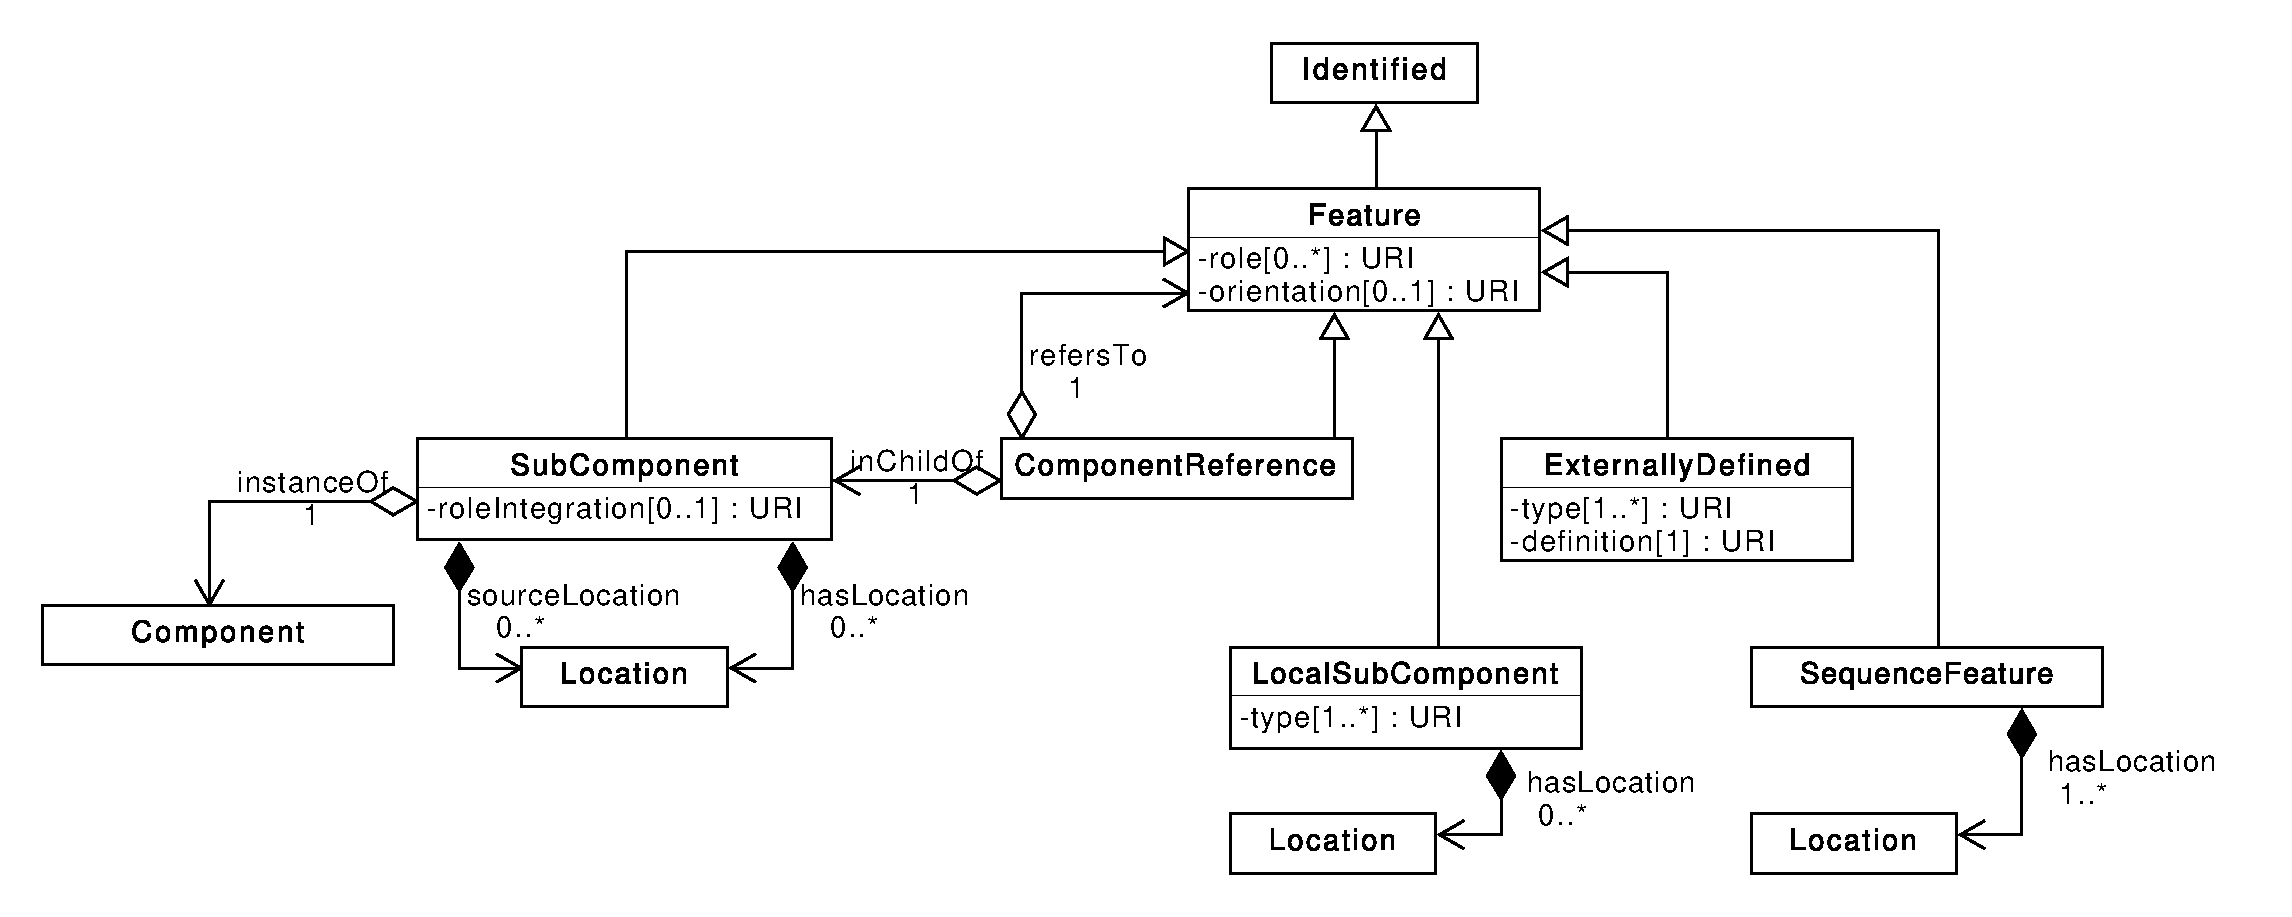
\includegraphics[width=\textwidth]{uml/feature}
\caption[]{Diagram of the \sbol{Feature} class, its children, and associated properties.}
\label{uml:subcomponent}
\end{center}
\end{figure}

\subparagraph{The \sbolheading{role} property}\label{sec:role:F}

Each \sbol{Feature} can have zero or more \sbolmult{role:F}{role} property \sbol{URI}s describing the purpose or potential function of this \sbol{Feature} in the \textit{context} of its parent \sbol{Component}.
If the \sbolmult{role:F}{role} for a \sbol{SubComponent} is left unspecified, then the \sbolmult{role:F}{role} is determined by the \sbolmult{role:C}{role} property of the \sbol{Component} that it is an \sbol{instanceOf}. 
If provided, these \sbolmult{role:F}{role} property \sbol{URI}s MUST identify terms from appropriate ontologies. Roles are not restricted to describing biological function; they may annotate a \sbol{Feature}'s function in any domain for which an ontology exists.
A table of recommended ontology terms for \sbolmult{role:F}{role} is given in \ref{tbl:component_roles}.

It is RECOMMENDED that these \sbolmult{role:F}{role} property \sbol{URI}s identify terms that are compatible with the \sbolmult{type:C}{type} properties of the \sbol{Feature}'s parent \sbol{Component}.
For example, a \sbolmult{role:F}{role} of a \sbol{Feature} which belongs to a \sbol{Component} of type DNA might refer to terms from the Sequence Ontology. 
Likewise, for any feature that is a \sbol{SubComponent}, the \sbolmult{role:F}{role} SHOULD be compatible with the \sbolmult{type:C}{type} of the \sbol{Component} that it links to through its \sbol{instanceOf} property.

\subparagraph{The \sbolheading{orientation} property}
\label{sec:orientation:F}
The \sbolmult{orientation:F}{orientation} property is OPTIONAL and has a data type of \sbol{URI}. This can be used to indicate how any associated double-stranded \sbol{Feature} is oriented on the \sbol{elements} of a \sbol{Sequence} from their parent \sbol{Component}. \ref{tbl:orientation_types} provides a list of REQUIRED \sbolmult{orientation:F}{orientation} \sbol{URI}s. If a \sbol{Feature} object has an \sbolmult{orientation:F}{orientation}, then it MUST come from \ref{tbl:orientation_types}.
 

\begin{table}[ht]
  \begin{edtable}{tabular}{lp{3.75in}}
    \toprule
    \textbf{Orientation URI} & \textbf{Description} \\
    \midrule
    \url{http://sbols.org/v3\#inline} & The region specified by this \sbol{Feature} or \sbol{Location} is on the \sbol{elements} of a \sbol{Sequence}. \\
    \url{http://sbols.org/v3\#reverseComplement} & The region specified by this \sbol{Feature} or \sbol{Location} is on the reverse-complement mapping of the \sbol{elements} of a \sbol{Sequence}. The exact nature of this mapping depends on the \sbol{encoding} of the \sbol{Sequence}. \\
    \bottomrule
  \end{edtable}
  \caption{REQUIRED \sbol{URI}s for the \sbolmult{orientation:F}{orientation} property}
  \label{tbl:orientation_types}
\end{table}

\paragraph{SubComponent}
\label{sec:SubComponent}

The \sbol{SubComponent} class is a subclass of the \sbol{Feature} class that can be used to specify structural hierarchy.
For example, the \sbol{Component} of a gene might contain four \sbol{SubComponent} objects: a promoter, RBS, CDS, and terminator, each linked to a \sbol{Component} that provides the complete definition.
In turn, the \sbol{Component} of the promoter \sbol{SubComponent} might itself contain \sbol{SubComponent} objects defining various operator sites, etc.

\subparagraph{The \sbolheading{roleIntegration} property}\label{sec:roleIntegration}

A \sbol{roleIntegration} specifies the relationship between a \sbol{SubComponent} instance's own set of \sbolmult{role:F}{role} properties and the set of \sbolmult{role:C}{role} properties on the included \sbol{Component}.

The \sbol{roleIntegration} property has a data type of \sbol{URI}. A \sbol{SubComponent} instance with zero \sbolmult{role:F}{role} properties MAY OPTIONALLY specify a \sbol{roleIntegration}. A \sbol{SubComponent} instance with one or more \sbolmult{role:F}{role} properties MUST specify a \sbol{roleIntegration} from \ref{tbl:component_roleIntegration}.
If zero \sbol{SubComponent} \sbolmult{role:F}{role} properties are given and no \sbol{SubComponent} \sbol{roleIntegration} is given, then \url{http://sbols.org/v3\#mergeRoles} is assumed.
It is RECOMMENDED to specify \sbol{SubComponent} \sbolmult{role:F}{role} values only if the result would differ from the  \sbolmult{role:C}{role} values belonging to this \sbol{SubComponent}'s included \sbol{Component}.

\begin{table}[ht]
  \begin{edtable}{tabular}{lp{4in}}
    \toprule
    \textbf{roleIntegration URI} & \textbf{Description} \\
    \midrule
    \url{http://sbols.org/v3\#overrideRoles} & In the context of this \sbol{SubComponent}, ignore any \sbolmult{role:C}{role} given for the included \sbol{Component}. Instead use only the set of zero or more \sbolmult{role:F}{role} properties given for this \sbol{SubComponent}. \\
    \url{http://sbols.org/v3\#mergeRoles} & Use the union of the two sets: both the set of zero or more \sbolmult{role:F}{role} properties given for this \sbol{SubComponent} as well as the set of zero or more \sbolmult{role:C}{role} properties given for the included \sbol{Component}. \\
    \bottomrule
  \end{edtable}
  \caption{Each \sbol{roleIntegration} mode is associated with a rule governing how a \sbol{SubComponent}'s \sbolmult{role:F}{role} values are to be combined with the included \sbol{Component}'s \sbolmult{role:C}{role} values.}
  \label{tbl:component_roleIntegration}
\end{table}

\subparagraph{The \sbolheading{instanceOf} property}
\label{sec:instanceOf}

The \sbol{instanceOf} property is a REQUIRED \sbol{URI} that refers to the \sbol{Component} providing the definition for this \sbol{SubComponent}.
Among other things, as described in the previous section, this \sbol{Component} effectively provides information about the \sbolmult{type:C}{type} and \sbolmult{role:C}{role} of the \sbol{SubComponent}.

The \sbol{instanceOf} property MUST NOT refer to the same \sbol{Component} as the one that contains the \sbol{SubComponent}.
Furthermore, \sbol{SubComponent} objects MUST NOT form a cyclical chain of references via their \sbol{instanceOf} properties and the \sbol{Component} objects that contain them.
For example, consider the \sbol{SubComponent} objects $A$ and $B$ and the \sbol{Component} objects $X$ and $Y$. The reference chain ``$X$ has feature $A$, $A$ is an instance of $Y$, $Y$ has feature $B$, and $B$ is an instance of $X$'' is cyclical.


\subparagraph{The \sbolheading{hasLocation} property}\label{sec:hasLocation:SC}

A \sbol{SubComponent} MAY have any number of \sbolmult{hasLocation:SC}{hasLocation} properties, each of type \sbol{URI}, that MUST refer to \sbol{Location} objects that indicates the location of the \sbol{Sequence} from the \sbol{instanceOf} \sbol{Component} in a \sbol{Sequence} of the parent \sbol{Component}.

If any \sbolmult{hasLocation:SC}{hasLocation} is defined, then there MUST BE precisely one \sbol{Sequence} in the \sbol{instanceOf} \sbol{Component}, as otherwise this relationship is ill-defined.

If no \sbolmult{hasLocation:SC}{hasLocation} is defined, this indicates a part / sub-part relationship for which sequence details have not (yet) been determined or involving types for which sequence relationships are not relevant (e.g., inclusion of a reaction chain within a larger metabolic network).

Allowing multiple \sbol{Location} objects on a single \sbol{SubComponent} is intended to enable representation of discontinuous regions (for example, a coding sequence encoded across a set of exons with interspersed introns).
As such, the \sbol{Location} objects of a single \sbol{SubComponent} MUST NOT specify overlapping regions, since it is not clear what this would mean.
There is no such concern with different objects, however, which can freely overlap in \sbol{Location} (for example, specifying overlapping linkers for sequence assembly).


\subparagraph{The \sbolheading{sourceLocation} property}\label{sec:sourceLocation}

The \sbol{sourceLocation} property allows for only a portion of a \sbol{Component}'s \sbol{Sequence} to be included, rather than its entirety.
For example, when composing parts with certain assembly methods, some bases on the boundary may be removed or replaced.
Another example is describing a deletion or replacement of a portion of a sequence.

A \sbol{SubComponent} MAY have any number of \sbol{sourceLocation} properties, each of type \sbol{URI}, that MUST refer to  \sbol{Location} objects that indicate which \sbol{elements} of the \sbol{instanceOf} \sbol{Component}'s \sbol{Sequence} are used in defining the parent of the \sbol{SubComponent}.

If there are no \sbol{sourceLocation} properties, then the whole \sbol{Sequence} is assumed to be included. 


\paragraph{ComponentReference}
\label{sec:ComponentReference}

The \sbol{ComponentReference} class is a subclass of \sbol{Feature} that can be used to reference \sbol{Feature}s within\\ \sbol{SubComponent}s. 

\subparagraph{The \sbolheading{inChildOf} property}\label{sec:inChildOf}

The \sbol{inChildOf} property is a REQUIRED \sbol{URI} that refers to a \sbol{SubComponent}. 
The \sbol{inChildOf} property MUST refer to a \sbol{SubComponent} pointed directly to by the parent of the \sbol{ComponentReference}.
Specifically:
\begin{itemize}
\item If the parent of the \sbol{ComponentReference} is a \sbol{Component}, then \sbol{inChildOf} MUST be one of its \sbol{SubComponent}s.
\item If the parent of the \sbol{ComponentReference} is another \sbol{ComponentReference}, then \sbol{inChildOf} MUST be a \sbol{SubComponent} of the \sbol{Component} linked as \sbol{instanceOf} the parent's \sbol{inChildOf} \sbol{SubComponent}.
\end{itemize}

\subparagraph{The \sbolheading{hasFeature} property}\label{sec:hasFeature:CR}

The \sbolmult{hasFeature:CR}{hasFeature} property is a REQUIRED \sbol{URI} that refers to a \sbol{Feature}.

This can be used to either link to the \sbol{Feature} being referenced or to chain hierarchically through additional layers of \sbol{SubComponent}.
\begin{itemize}
\item If the \sbol{Feature} is a \sbol{ComponentReference}, then that \sbol{ComponentReference} acts as a hierarchical link in a chain of references, and MUST be either a child of the \sbol{ComponentReference} linking to it via \sbolmult{hasFeature:CR}{hasFeature} or a child of the \sbol{Component} linked as \sbol{instanceOf} the \sbol{ComponentReference}'s \sbol{inChildOf} \sbol{SubComponent}.
\item Otherwise, if the \sbol{hasFeature} refers to any other type of \sbol{Feature}, that \sbol{Feature} MUST be a child of the \sbol{Component} linked as \sbol{instanceOf} the \sbol{ComponentReference}'s \sbol{inChildOf} \sbol{SubComponent}.
\end{itemize}

For example, \sbol{ComponentReference} R1 looking into a \sbol{SubComponent} for a plasmid might link with \sbol{hasFeature} to its own child \sbol{ComponentReference} R2, which in turn looks within the \sbol{Component} defining the plasmid to the plasmid's CDS \sbol{SubComponent}, in turn using \sbol{hasFeature} to reference a \sbol{SequenceFeature} within the \sbol{Component} that defines that CDS.



\paragraph{LocalSubComponent}
\label{sec:LocalSubComponent}

The \sbol{LocalSubComponent} class is a subclass of \sbol{Feature}. 
This class serves as a way to create a placeholder in more complex \sbol{Component}s, such as a variable to be filled in later or a composite that exists only within the context of the parent \sbol{Component}.

\subparagraph{The \sbolheading{hasLocation} property}\label{sec:hasLocation:LSR}

A \sbol{LocalSubComponent} MAY have any number of \sbolmult{hasLocation:LSR}{hasLocation} properties, each of type \sbol{URI}, that MUST refer to \sbol{Location} objects. 
These follow the same restrictions as for the \sbolmult{hasLocation:SC}{hasLocation} of a \sbol{SubComponent}, notably that the \sbol{Location}s of \sbolmult{hasLocation:LSR}{hasLocation} properties attached to the same \sbol{LocalSubComponent} MUST NOT overlap.


\subparagraph{The \sbolheading{type} property}\label{sec:type:LSC}

The \sbolmult{type:LSC}{type} property is REQUIRED and contains one or more \sbol{URI}s. The \sbolmult{type:LSC}{type} property is identical to its use in \sbol{Component}.

\paragraph{ExternallyDefined}
\label{sec:ExternallyDefined}

The \sbol{ExternallyDefined} class has been introduced so that external definitions in databases like ChEBI or UniProt can be referenced.

\subparagraph{The \sbolheading{type} property}\label{sec:type:ED}

The \sbolmult{type:ED}{type} property is REQUIRED and contains one or more \sbol{URI}s. The \sbolmult{type:ED}{type} property is identical to its use in \sbol{Component}.

\subparagraph{The \sbolheading{definition} property}\label{sec:definition:ER}

The \sbolmult{definition:ER}{definition} property is REQUIRED and is of type \sbol{URI} that links to a canonical definition external to SBOL.
When possible, such definitions SHOULD use the recommended external resources in \ref{sec:recomm_ontologies}.
For example, an \sbol{ExternallyDefined} simple chemical might link to ChEBI and a protein might link to UniProt.


\paragraph{SequenceFeature}
\label{sec:SequenceFeature}

The \sbol{SequenceFeature} class describes one or more regions of interest on the \sbol{Sequence} objects referred to by its parent \sbol{Component}. 

\subparagraph{The \sbolheading{hasLocation} property}\label{sec:hasLocation:SF}

A \sbol{SequenceFeature} MAY have any number of \sbolmult{hasLocation:SF}{hasLocation} properties, each of type \sbol{URI}, that MUST refer to \sbol{Location} objects. 
These follow the same restrictions as for the \sbolmult{hasLocation:SC}{hasLocation} of a \sbol{SubComponent}, notably that the \sbol{Location}s of \sbolmult{hasLocation:SF}{hasLocation} properties attached to the same \sbol{SequenceFeature} MUST NOT overlap.

